
\begin{abstract}
\noindent Kolmogorov complexity ($K$) is an incomputable function. It can be approximated from above but not to arbitrary given precision and it cannot be approximated from below. By restricting the source of the data to a specific model class, we can construct a computable function $\ok$ to approximate $K$ in a probabilistic sense: the probability that the error is greater than $k$ decays exponentially with $k$. We apply the same method to the normalized information distance (NID) and discuss conditions that affect the safety of the approximation.
\end{abstract}

\noindent The Kolmogorov complexity of an object is its shortest description, considering all computable descriptions. It has been described as ``the accepted absolute measure of information content of an individual object'' \cite{DBLP:journals/tit/GacsTV01}, and its investigation has spawned a slew of derived functions and analytical tools. Most of these tend to separate neatly into one of two categories: the platonic and the practical. 

On the platonic side, we find such tools as the normalized information distance \cite{DBLP:journals/tit/LiCLMV04}, algoritheoremic statistics \cite{DBLP:journals/tit/GacsTV01} and sophistication \cite{DBLP:journals/tit/Vitanyi06,adriaans2012facticity}. These subjects all deal with incomputable ``ideal'' functions: they optimize over all computable functions, but they cannot be computed themselves.

To construct practical applications (ie. runnable computer programs), the most common approach is to take one of these platonic, incomputable functions, derived from Kolmogorov complexity ($K$), and to approximate it by swapping $K$ out for a computable compressor like GZIP \cite{gailly1991gzip}. This approach has proved effective in the case of normalized information distance (NID) \cite{DBLP:journals/tit/LiCLMV04} and its approximation, the normalized compression distance (NCD) \cite{DBLP:journals/tit/CilibrasiV05}. Unfortunately, the switch to a general-purpose compressor leaves an analytical gap. We know that the compressor serves as an upper bound to $K$---up to a constant---but we do not know the difference between the two, and how this error affects the error of derived functions like the NCD. This can cause serious contradictions. For instance, the normalized information distance has been shown to be non-approximable \cite{DBLP:journals/jcss/TerwijnTV11}, yet the NCD has proved its merit empirically \cite{DBLP:journals/tit/CilibrasiV05}. Why this should be the case, and when this approach may fail has, to our knowledge, not yet been investigated.

We aim to provide the first tools to bridge this gap. We will define a computable function which can be said to approximate Kolmogorov complexity, with some practical limit to the error. To this end, we introduce two concepts:

\begin{itemize}
\item We generalize resource-bounded Kolmogorov complexity ($K^t$) to \emph{model-\\bounded Kolmogorov complexity}, which minimizes an object's description length over any given enumerable subset of Turing machines (a \emph{model class}). We explicitly assume that the source of the data is contained in the model class. 
\item We introduce a probabilistic notion of approximation. A function approximates another \emph{safely}, under a given distribution, if the probability of them differing by more than $k$ bits, decays at least exponentially in $k$. \footnotemark
\end{itemize}

\footnotetext{This consideration is subject to all the normal drawbacks of asymptotic approaches. For this reason, we have foregone the use of big-O notation as much as possible, in order to make the constants and their meaning explicit.} 

\noindent While the resource-bounded Kolmogorov complexity is computable in a technical sense, it is never computed practically. The generalization to model bounded Kolmogorov complexity creates a connection to \emph{minimum description length} (MDL) \cite{rissanen1978modeling,DBLP:journals/tit/Rissanen84,grunwald2007minimum}, which does produce algoritheorems and methods that are used in a practical manner. Kolmogorov complexity has long been seen as a kind of platonic ideal which MDL approximates. Our results show that MDL is not just an upper bound to $K$, it also approximates it in a probabilistic sense.

Interestingly, the model-bounded Kolmogorov complexity itself---the smallest description using a single element from the model class---is not a safe approximation. We can, however, construct a computable, safe approximation by taking into account all descriptions the model class provides for the data.

The main result of this paper is a computable function $\ok$ which, under a model assumption, safely approximates $K$ (Theorem~\ref{theorem:safe-computable}). We also investigate whether a $\ok$-based approximation of NID is safe, for different properties of the model class from which the data originated (Theorems \ref{theorem:unsafe-id}, \ref{theorem:safe-id} and \ref{theorem:safe-nid}).


\section{Turing Machines and Probability}

\subsection*{Turing Machines}

Let $\B= \{0, 1\}^*$. We assume that our data is encoded as a finite binary string. Specifically, the natural numbers can be associated to binary strings, for instance by the bijection: $(0, \epsilon)$, $(1, 0)$, $(2, 1)$, $(3, 00)$, $(4, 01)$, etc, where $\epsilon$ is the empty string. To simplify notation, we will sometimes conflate natural numbers and binary strings, implicitly using this ordering.

We fix a canonical prefix-free coding, denoted by $\overline{x}$, such that $|\overline{x}| \leq |x| + 2 \log{|x|}$. See \cite[Example~1.11.13]{DBLP:books/daglib/0087328} for an example . Among other things, this gives us a canonical pairing function to encode two strings $x$ and $y$ into one: $\overline{x}y$.

\noindent We use the Turing machine model from \cite[Example~3.1.1]{DBLP:books/daglib/0087328}. The following properties are important: the machine has a read-only, right-moving input tape, an auxiliary tape which is read-only and two-way, two read-write two-way worktapes and a read-write two-way output tape.\footnotemark~All tapes are one-way infinite. If a tape head moves off the tape or the machine reads beyond the length of the input, it enters an infinite loop. For the function computed by TM $i$ on input $p$ with auxiliary input $y$, we write $T_i(p\mid y)$ and $T_i(p) = T_i(p \mid \epsilon)$. The most important consequence of this construction is that the programs for which a machine with a given auxiliary input $y$ halts, form a prefix-free set \cite[Example~3.1.1]{DBLP:books/daglib/0087328}. This allows us to interpret the machine as a probability distribution (as described in the next subsection).

\footnotetext{Multiple work tapes are only required for proofs involving resource bounds.}

We fix an effective ordering $\{T_i\}$. We call the set of all Turing machines $\C$. There exists a universal Turing machine, which we will call $U$, that has the property that $U(\overline{\imath}p\mid y) = T_i(p\mid y)$ \cite[Theorem~3.1.1]{DBLP:books/daglib/0087328}. 

\subsection*{Probability}

We want to formalize the idea of a probability distribution that is \emph{computable}: it can be simulated or computed by a computational process. For this purpose, we will interpret a given Turing machine $T_q$ as a probability distribution $p_q$: each time the machine reads from the input tape, we provide it with a random bit. The Turing machine will either halt, read a finite number of bits without halting, or read an unbounded number of bits. $p_q(x)$ is the probability that this process halts and produces $x$: $p_q(x) = \sum_{p: T_q(p) = x} 2^{-|p|}$. We say that $T_q$ \emph{samples} $p_q$. Note that if $p$ is a semimeasure, $1-\sum_x p(x)$ corresponds to the probability that this sampling process will not halt.

We model the probability of $x$ conditional on $y$ by a Turing machine with $y$ on its auxiliary tape: $p_q(x \mid y) = \sum_{p : T_q(p|y) = x} 2^{-|p|}$.  

The \emph{lower semicomputable semimeasures} \cite[Chapter~4]{DBLP:books/daglib/0087328} are an alternative formalization. We show that it is equivalent to ours:

\renewcommand*{\thefootnote}{\fnsymbol{footnote}}

\begin{lemma}\footnotemark[2]
The set of probability distributions sampled by Turing machines in $\C$ is equivalent to the set of lower semicomputable semimeasures.
\label{lemma:sampling-equivalence}
\end{lemma}

\footnotetext[2]{Proof in the appendix.}

\noindent The distribution corresponding to the universal Turing machine $U$ is called $m$: $m(x) = \sum_{p: U(p) = x} 2^{-|p|}$. This is known as a universal distribution. $K$ and $m$ dominate each other, ie. $\exists c \forall x : |K(x) - \log m(x)| < c$ \cite[Theorem~4.3.3]{DBLP:books/daglib/0087328}.

\section{Model-Bounded Kolmogorov Complexity}

In this section we present a generalization of the notion of resource-bounded Kolmogorov complexity. We first review the unbounded version:

\begin{definition}
Let $k(x\mid y) = \argmin_{p:U(p\mid y) = x} |p|$. The prefix-free, conditional \emph{Kolmogorov complexity} is \begin{align*}
K(x\mid y) = |k(x\mid y)|
\end{align*} with $K(x) = K(x\mid \epsilon)$. \label{definition:kolmogorov-complexity}
\end{definition}
Due to the halting problem, $K$ is not computable. By limiting the set of Turing machines under consideration, we can create a computable approximation. 

\begin{definition}
A \emph{model class} $C \subseteq \C$ is a computably enumerable set of Turing machines. Its members are called \emph{models}. A \emph{universal model} for $C$ is a Turing machine $U^C$ such that $U^C(\overline{\imath}p\mid y) = T_i(p\mid y)$ where $i$ is an index over the elements of $C$. 
\end{definition}

\begin{definition}
For a given $C$ and $U^C$ we have $K^C(x) = \min \left \{|p| \;:\; U^C(p) = x \right \}$, called the \emph{model-bounded Kolmogorov complexity}.
\end{definition}
$K^C$, unlike $K$, depends heavily on the choice of enumeration of $C$. A notation like $K_{U^C}$ or $K^{i, C}$ would express this dependence better, but for the sake of clarity we will use $K^C$.

We define a model-bounded variant of $m$ as $m^C(x) = \sum_{p: U^C(p) = x} 2^{-|p|}$, which dominates all distributions in $C$:

\begin{lemma}
For any $T_q \in C$, $m^C(x) \geq c_q p_q(x)$ for some $c_q$ independent of $x$.
\label{lemma:universal-bounded-distribution}
\end{lemma}
\begin{proof}\belowdisplayskip=-12pt
\begin{align*}
m^C(x) = \sum_{i,p : U^C(\overline{\imath}p) = x} 2^{-|\overline{\imath}p|} 
\geq \sum_{p : U^C(\overline{q}p) = x} 2^{-|\overline{q}|}2^{-|p|} 
= 2^{-|\overline{q}|} p_q(x) \p
\end{align*}
\end{proof}

\noindent Unlike $K$ and $-\log m$, $K^C$ and $-\log m^C$ do not dominate one another. We can only show that $-\log m^C$ bounds $K^C$ from below ($\sum_{U^C(p)=x} 2^{-|p|} > 2^{-|k^C(x)|}$). In fact, as shown in Theorem~\ref{theorem:unsafe}, $-\log m^C$ and $K^C$ can differ by arbitrary amounts.

\renewcommand*{\thefootnote}{\arabic{footnote}}

\begin{example}[{resource-bounded Kolmogorov complexity \cite[Ch.~7]{DBLP:books/daglib/0087328}}]
\label{example:traditional-time-bounded}
\-\\ Let $t(n)$ be some time-constructible function.\footnotemark Let $T_i^t$ be the modification of $T_i \in \C$ such that at any point in the computation, it halts immediately if more than $k$ cells have been written to on the output tape and the number of steps that have passed is less than $t(k)$. In this case, whatever is on the output tape is taken as the output of the computation. If this situation does not occur, $T_i$ runs as normal. Let $U^t(\overline{\imath}p) = T^t_i(p)$. We call this model class $C^t$. We abbreviate $K^{C^t}$ as $K^t$. 

Since there is no known means of simulating $U^t$ within $t(n)$, we do not know whether $U^t \in C^t$. It can be run in $ct(n) \log t(n)$ \cite{DBLP:books/daglib/0087328,DBLP:journals/jacm/HennieS66}, so we do know that $U^t \in C^{ct\log t}$.
\end{example}

\footnotetext{Ie. $t: \N \rightarrow \N$ and $t$ can be computed in $O(t(n))$~\cite{DBLP:journals/mst/AntunesMSV09}.}

\noindent Other model classes include Deterministic Finite Automata, Markov Chains, or the exponential family (suitably discretized). These have all been thoroughly investigated in coding contexts in the field of Minimum Description Length \cite{grunwald2007minimum}.

\renewcommand*{\thefootnote}{\fnsymbol{footnote}}

\section{Safe Approximation}

When a code-length function like $K$ turns out to be incomputable, we may try to find a lower and upper bound, or to find a function which dominates it. Unfortunately, neither of these will help us. Such functions invariably turn out to be incomputable themselves \cite[Section~2.3]{DBLP:books/daglib/0087328}. 

To bridge the gap between incomputable and computable functions, we require a softer notion of approximation; one which states that errors of any size may occur, but that the larger errors are so unlikely, that they can be safely ignored: 

\begin{definition}
Let $f$ and $f_a$ be two functions. We take $f_a$ to be an approximation of $f$. We call the approximation \emph{$b$-safe (from above)} for a distribution (or \emph{adversary}) $p$ if for all $k$ and some $c > 0$: 
\[
p(f_a(x) - f(x) \geq k) \leq c b^{-k} \p
\] 
Since we focus on code-length functions, usually omit ``from above''. A \emph{safe} function is $b$-safe for some $b > 1$. An approximation is safe for a model class $C$ if it is safe for all $p_q$ with $T_q \in C$.
\label{definition:safety}
\end{definition}

\noindent While the definition requires this property to hold for all $k$, it actually suffices to show that it holds for $k$ above a constant, as we can freely scale $c$:

\begin{lemma}
If $\exists_{c} \forall_{k: k >k_0} : p(f_a(x) - f(x) \geq k) \leq c b^{-k}$, then $f_a$ is $b$-safe for $f$ against $p$. \label{lemma:k-zero}
\end{lemma}
\begin{proof}
First, we name the $k$ below $k_0$ for which the ratio between the bound and the probability is the greatest: $k_m = \argmax_{k\in [0, k_0]} \left[p(f_a(x) - f(x) \geq k)/cb^{-k}\right]$. We also define $b_m = cb^{-k_m}$ and $p_m = p(f_a(x) - f(x) \geq k_m)$. At $k_m$, we have $p(f_a(x) - f(x)\geq k_m) = p_m = \frac{p_m}{b_m}cb^{-k_m}$. In other words, the bound $c'b^{-k}$ with $c' = \frac{p_m}{b_m}c$ bounds $p$ at $k_m$, the point where it diverges the most from the old bound. Therefore, it must bound it at all other $k >0$ as well.
\end{proof}

\noindent Safe approximation, domination and lowerbounding form a hierarchy:

\begin{lemma}
Let $f_a$ and $f$ be code-length functions. If $f_a$ is a lower bound on $f$, it also dominates $f$. If $f_a$ dominates $f$, it is also a safe approximation.
\label{lemma:domination-safety}
\end{lemma}
\begin{proof}
Domination means that for all $x$: $f_a(x) - f(x) < c$, if $f_a$ is a lower bound, $c=0$. If $f_a$ dominates $f$ we have  
$\forall p, k > c : p(f_a(x) - f(x) \geq k) = 0$.
\end{proof}
Finally, we show that safe approximation is transitive, so we can chain together proofs of safe approximation; if we have several functions with each safe for the next, we know that the first is also safe for the last.

\begin{lemma}
The property of safety is transitive over the space of functions from $\mathbb B$ to $\mathbb B$ for a fixed adversary.
\label{lemma:reflexitvity}
\end{lemma}
\begin{proof} Let $f$, $g$ and $h$ be functions such that 
\begin{align*}
p(f(x) - g(x) \geq k) &\leq c_1{b_1}^{-k} \text{ and}\\
p(g(x) - h(x) \geq k) &\leq c_2{b_2}^{-k} \p
\end{align*}
We need to show that $p(f(x) - h(x) \geq k)$ decays exponentially with $k$. We start with
\begin{align*}
p\left(f(x) - g(x) \geq k \vee g(x) - h(x) \geq k\right)\;&\leq\;c_1{b_1}^{-k} + c_2{b_2}^{-k}\p
\end{align*}
$\left\{x : f(x) - h(x) \geq 2k\right\}$ is a subset of $\left\{x : f(x) - g(x) \geq k\vee g(x) - h(x) \geq k\right\}$, so that the probability of the first set is less than that of the second:
\begin{align*}
p\left(f(x) - h(x) \geq 2k\right) \leq c_1{b_1}^{-k} + c_2{b_2}^{-k} \p
\end{align*}
Which gives us \belowdisplayskip=-12pt
\begin{align*}
&p\left(f(x) - h(x) \geq 2k\right)\leq cb^{-k} \quad&& \text{with $b=\min(b_1, b_2)$ and $c = \max(c_1, c_2)$} \;,\\
&p\left(f(x) - h(x) \geq k'\right)\leq cb'^{-k'} \quad&& \text{with $b'=\sqrt{b}$}\p
\end{align*} 
\end{proof}

\section{A Safe, Computable Approximation of $K$}

\begin{figure*}[tb]
  \centering
  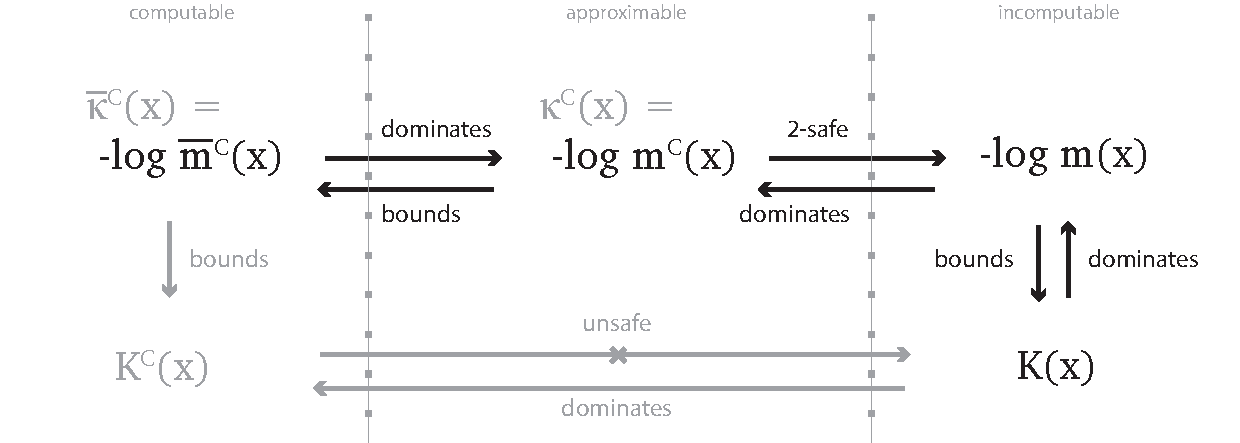
\includegraphics[width=\textwidth]{./images/approximation-map.pdf}
  \caption{\small An overview of how various code-length functions relate to each other in terms of approximation safety. These relations hold under the assumption that the data is generated by a distribution in $C$ and that $C$ is sufficient and complete.}
  \label{fig:approximation-map}
\end{figure*}

Assuming that our data is produced from a model in $C$, can we construct a computable function which is safe for $K$? An obvious first choice is $K^C$. For it to be computable, we would normally ensure that all programs for all models in $C$ halt. Since the halting programs form a prefix-free set, this is impossible. There is however a property for prefix-free functions that is analogous. We call this \emph{sufficiency}:

\begin{definition}
A sufficient model $T$ is a model for which every infinite binary string contains a halting program as a prefix. A \emph{sufficient model class} contains only sufficient models. 
\end{definition}
We can therefore enumerate all inputs for $U^C$ from short to long in series to find $k^C(x)$, so long as $C$ is sufficient. For each input, $U^C$ either halts or attempts to read beyond the length of the input. 

In certain cases, we also require that $C$ can represent all $x \in \B$ (ie. $m^C(x)$ is never 0). We call this property \emph{completeness}:
\begin{definition}
A model class $C$ is called \emph{complete} if for any $x$, there is at least one $p$ such that $U^C(p) = x$. 
\end{definition}
We can now say, for instance, that $K^C$ is computable for sufficient $C$. Unfortunately, $K^C$ turns out to be unsafe:
\begin{theorem}
There exist model classes $C$ so that $K^C(x)$ is an unsafe approximation for $K(x)$ against some $p_q$ with $T_q \in C$.  \label{theorem:unsafe}
\end{theorem}
\begin{proof}
We first show that $K^C$ is unsafe for $-\log m^C$. 

Let $C$ contain a single Turing machine $T_q$ which outputs $x$ for any input of the form $\overline{x}p$ with $|p| = x$ and computes indefinitely for all other inputs.

$T_q$ samples from $p_q(x) = 2^{-|\overline{x}|}$, but it distributes each $x$'s probability mass uniformly over many programs much longer than $|\overline{x}|$.

This gives us $K^C(x) = |\overline{x}| + |p| = |\overline{x}| + x $ and $-\log m^C(x) = |\overline{x}|$, so that $K^C(x) + \log m^C(x) = x$. We get 
\begin{align*}
m^C&(K^C(x) + \log m^C(x) \geq k) = m^C(x \geq k) = \\
&\sum_{x : x \geq k} 2^{-|\overline{x}|} \geq \sum_{x : x \geq k} 2^{-2 \log x} \geq k^{-2}
\end{align*}
so that $K^C$ is unsafe for $-\log m^C$.

It remains to show that this implies that $K^C$ is unsafe for $K$. In Theorem~\ref{theorem:safe}, we prove that $-\log m^C$ is safe for $K$. Assuming that $K^C$ is safe for $K$ (which dominates $-\log m^C$) implies $K^C$ is safe for $-\log m^C$, which gives us a contradiction.
\end{proof}
Note that the use of a model class with a single model is for convenience only. The main requirement for $K^C$ to be unsafe is that the prefix tree of $U^C$'s programs distributes the probability mass for $x$ over many programs of similar length. The greater the difference between $K^C$ and $- \log m^C$, the greater the likelihood that $K^C$ is unsafe.

Our next candidate for a safe approximation of $K$ is $-\log m^C$. This time, we fare better. We first require the following lemma, called the \emph{no-hypercompression theorem} in \cite[p103]{grunwald2007minimum}:
\begin{lemma}
Let $p_q$ be a probability distribution. The corresponding code-length function, $-\log p_q$, is a $2$-safe approximation for any other code-length function against $p_q$. For any $p_r$ and $k>0$: $
p_q(-\log p_q(x) +  \log p_r(x) \geq k) \leq 2^{-k}$.
\label{lemma:no-hypercompression}
\end{lemma} 

\renewcommand*{\thefootnote}{\arabic{footnote}}

\begin{theorem}
$-\log m^C(x)$ is a 2-safe approximation of $K(x)$ against any adversary from $C$.
\label{theorem:safe}
\end{theorem}
\begin{proof}\belowdisplayskip=-12pt
Let $p_q$ be some adversary in $C$. We have 
\begin{align*}
p_q&(-\log m^C(x) - K(x) \geq k) \\ 
&\leq c m^C(-\log m^C(x) - K(x) \geq k) &\text{by Lemma~\ref{lemma:universal-bounded-distribution},} \\
&\leq c 2^{-k} &\text{by Lemma~\ref{lemma:no-hypercompression}.}
\end{align*}
\end{proof}
While we have shown $m^C$ to be safe for $K$, it may not be computable, even if $C$ is sufficient (since it is an infinite sum). We can, however, define an approximation, which, for sufficient $C$, is computable and dominates $m^C$.

\begin{definition}
\label{definition:algoritheorem}
Let the model class $D$ be the union of $C$ and some arbitrary sufficient and complete distribution from $\C$.

Let $\m^C_c(x)$ be the function computed by the following algoritheorem:
Dovetail the computation of all programs on $U^D(x)$ in cycles, so that in cycle $n$, the first $n$ programs are simulated for one further step. After each such step we consider the probability mass $s$ of all programs that have stopped (where each program $p$ contributes $2^{-|p|}$), and the probability mass $s_x$ of all programs that have stopped and produced $x$. We halt the dovetailing and output $s_x$ if $s_x > 0$ and the following stop condition is met:
\[
\frac{1-s}{s_x} \leq 2^c - 1 \p
\] 
\end{definition}
Note that if $C$ is sufficient so is $D$, so that $s$ goes to 1 and $s_x$ never decreases.  Since all programs halt, the stop condition must be reached. The addition of a complete model is required to ensure that $s_x$ does not remain $0$ indefinitely.

\begin{lemma}
If $C$ is sufficient, $\m^C_c(x)$ dominates $m^C$ with a constant multiplicative factor $2^{-c}$ (ie. their code-lengths differ by at most $c$ bits).
\label{lemma:overline-dominance}
\end{lemma}
\begin{proof}\belowdisplayskip=-12pt
We will first show that $\m^C_c$ dominates $m^D$. Note that when the computation of $\m^C_c$ halts, we have $\m^C_c(x) = s_x$ and $m^D(x) \leq s_x + (1 - s)$. This gives us:
\[
\frac{m^D(x)}{\m^C_c(x)} \leq 1 + \frac{1 - s}{s_x} \leq 2^{c} \p
\]
Since $C \subseteq D$, $m^D$ dominates $m^C$ (see Lemma~\ref{lemma:subset-dominance} in the appendix) and thus, $\m^C_c$ dominates $m^C$.
\end{proof}
The parameter $c$ in $\m^C_c$ allows us to tune the algoritheorem to trade off running time for a smaller constant of domination. We will usually omit it when it is not relevant to the context. 

Putting all this together, we have achieved our aim: 
\begin{theorem}
For a sufficient model class $C$, $-\log \overline{m}^C$ is a safe, computable approximation of $K(x)$ against any adversary from $C$
\label{theorem:safe-computable}
\end{theorem}
\begin{proof}
We have shown that, under these conditions, $-\log m^C$ safely approximates $-\log m$ which dominates $K$, and that $-\log \overline{m}^C$ dominates $-\log m^C$. Since domination implies safe approximation (Lemma~\ref{lemma:domination-safety}), and safe approximation is transitive (Lemma~\ref{lemma:reflexitvity}), we have proved the theorem.  
\end{proof}
Figure~\ref{fig:approximation-map} summarizes this chain of reasoning and other relations between the various code-length functions mentioned.

The negative logaritheorem of $m^C$ will be our go-to approximation of $K$, so we will abbreviate it with $\kappa$:
\begin{definition}
$\kappa^C(x) = -\log m^C(x)$ and $\ok^C(x) = -\log \m^C(x)$.
\end{definition}  
Finally, if we violate our model assumption we lose the property of safety. For adversaries outside $C$, we cannot be sure that $\kappa^C$ is safe:

\begin{theorem} 
There exist adversaries $p_q$ with $T_q \notin C$ for which neither $\kappa^C$ nor $\ok^C$ is a safe approximation of $K$. 
\label{theorem:unsafe-outside}
\end{theorem}
\begin{proof}
Consider the following algoritheorem for sampling from a computable distribution (which we will call $p_q$):
\begin{itemize}
\item Sample $n \in {\mathbb N}$ from some distribution $s(n)$ which decays polynomially. 
\item Loop over all $x$ of length $n$ return the first $x$ such that $\kappa^C(x) \geq n$. 
\end{itemize}
Note that at least one such $x$ must exist by a counting argument: if all $x$ of length $n$ have  $-\log \overline{m}^C(x) < n$ we have a code that assigns $2^n$ different strings to $2^n-1$ different codes.

For each $x$ sampled from $q$, we know that $\ok(x) \geq |x|$ and $K(x) \leq -\log p_q(x) + c_q$. Thus: 
\begin{align*}
p_q&(\ok^C(x) - K(x) \geq k) \;\geq\; p_q(|x| + \log p_q(x) - c_q \geq k) \\
&= p_q(|x| + \log s(|x|) - c_q \geq k) \;=\; \sum\nolimits_{n:n + \log s(n) - c_q \geq k} s(n)\p
\end{align*}
Let $n_0$ be the smallest $n$ for which $2n > n + \log s(n) - c_q$. For all $k > 2n_0$ we have \belowdisplayskip=-12pt
\begin{align*}
\sum\nolimits_{n:n + \log s(n) - c_q \geq k} s(n) \geq \sum\nolimits_{n: 2n \geq k} s(n) \geq s\left(\tfrac{1}{2} k\right)\p
\end{align*}
\end{proof}
For $C^t$ (as in Example~\ref{example:traditional-time-bounded}), we can sample the $p_q$ constructed in the proof in $O(2^n\cdot t(n))$. Thus, we know that $\kappa^t$ is safe for $K$ against adversaries from $C^t$, and we know that it is unsafe against $C^{2^t}$.
\section{Approximating Normalized Information Distance}

\begin{definition}[{\cite{DBLP:journals/tit/LiCLMV04,DBLP:journals/tit/CilibrasiV05}}]
The normalized information distance between two strings $x$ and $y$ is 
\[
\text{NID}(x, y) = \frac{\max \left [ K(x\mid y), K(y\mid x)\right ]}{\max \left [K(x), K(y)\right ]} \p
\]
\label{definition:nid}
\end{definition}
The information distance (ID) is the numerator of this function. The NID is neither lower nor upper semicomputable \cite{DBLP:journals/jcss/TerwijnTV11}. Here, we investigate whether we can safely approximate either function using $\kappa$. We define $\id^C$ and $\nid^C$ as the $\id$ and $\nid$ functions with $K$ replaced by $\ok^C$. We first show that, even if the adversary only combines functions and distributions in $C$, $\id^C$ may be an unsafe approximation.

\renewcommand*{\thefootnote}{\arabic{footnote}}
 
\begin{definition}\footnotemark
A function $f$ is a ($b$-safe) \emph{model-bounded one-way function} for $C$ if it is injective, and for some $b > 1$, some $c > 0$, all $q \in C$ and all $k$: 
\begin{align*}
p_q\left (\kappa^C(x) - \kappa^C\left(x\mid f(x)\right ) \geq k\right ) \leq cb^{-k} \p
\end{align*}
\label{definition:one-way}
\end{definition}

\footnotetext{This is similar to the Kolmogorov one-way function \cite[Definition~11]{DBLP:journals/mst/AntunesMPST13}.}
\renewcommand*{\thefootnote}{\fnsymbol{footnote}}

\begin{theorem}\footnotemark[2]
\label{theorem:unsafe-id}
Under the following assumptions:
\begin{itemize}
\item $C$ contains a model $T_0$, with $p_0(x) = 2^{-|x|}s(|x|)$, with $s$ a distribution on $\mathbb N$ which decays polynomially or slower,
\item there exists a model-bounded one-way function $f$ for $C$,
\item $C$ is \emph{normal}, ie. for some $c$ and all $x$: $\kappa^C(x) <  |\overline{x}| + c$
\end{itemize}
$\id^C$ is an unsafe approximation for $\id$ against an adversary $T_q$ which samples $x$ from $p_0$ and returns $\overline{x}f(x)$.
\end{theorem}
If $x$ and $y$ are sampled from $C$ independently, we can prove safety:

\begin{theorem}\footnotemark[2]
Let $T_q$ be a Turing machine which samples $x$ from $p_a$, $y$ from $p_b$ and returns $\overline{x}y$. If $T_a, T_b \in C$, $\id^C(x, y)$ is a safe approximation for $\id(x, y)$ against any such $T_q$.
\label{theorem:safe-id}    
\end{theorem}
The proof relies on two facts:
\begin{itemize}
  \item $\ok^C(x\mid y)$ is safe for $K(x\mid y)$ if $x$ and $y$ are generated this way.
  \item  Maximization is a \emph{safety preserving operation}: if we have two functions $f$ and $g$ with safe approximations $f_a$ and $g_a$, $\max(f_a(x), g_a(x))$ is a safe approximation of $\max(f(x), g(x))$.
\end{itemize} 
For \emph{normalized} information distance, which is dimensionless, the error $k$ in bits as we have used it so far does not mean much. Instead, we use  $f/f_a$ as a measure of approximation error, and we introduce an additional parameter $\epsilon$:

\begin{theorem}\footnotemark[2]
We can approximate $\nid$ with $\nid^C$ with the following bound:
\[
p_q\left(\frac{\nid(x, y)}{\nid^C(x, y)} \notin \left (1 - \frac{k}{c}, 1 + \frac{k}{c}\right ) \right) \leq c'b^{-k} + 2\epsilon
\]
with 
\begin{align*}
p_q(\text{\textnormal{ID}}^C(x, y) \geq c) \leq \epsilon \;\text{and}\; p_q\left(\max \left[\kappa^C(x), \kappa^C(y)\right] \geq c\right) \leq \epsilon
\end{align*}
for some $b > 1$ and $c' > 0$, assuming that $p_q$ samples $x$ and $y$ independently from models in $C$.
\label{theorem:safe-nid}
\end{theorem}

\section{Discussion}

We have provided a function $\ok^C(x)$ for a given model class $C$, which is computable if $C$ is sufficient. Under the assumption that $x$ is produced by a model from $C$, $\ok^C(x)$ approximates $K(x)$ in a probabilistic sense. We have also shown that $K^C(x)$ is not safe. Finally, we have given some insight into the conditions on $C$ and the adversary, which can affect the safety of NCD as an approximation to NID.

Since, as shown in Example~\ref{example:traditional-time-bounded}, resource-bounded Kolmogorov complexity is a variant of model-bounded Kolmogorov complexity, our results apply to $K^t$ as well: $K^t$ is not necessarily a safe approximation of $K$, even if the data can be sampled in $t$ and $\kappa^t$ \emph{is} safe if the data can be sampled in $t$. Whether $K^t$ is safe ultimately depends on whether a single shortest program dominates among the sum of all programs, as it does in the unbounded case.

For complex model classes, $\kappa^C$ may still be impractical to compute. In such cases, we may be able to continue the chain of safe approximation proofs. Ideally, we would show that a model which is only locally optimal, found by an iterative method like gradient descent, is still a safe approximation of $K$. Such proofs would truly close the circuit between the ideal world of Kolmogorov complexity and modern statistical practice.

\section{Appendix}
\renewcommand*{\thefootnote}{\arabic{footnote}} 

\subsection{Turing Machines and lsc. Probability Semimeasures (Lemma~\ref{lemma:sampling-equivalence})} 
\begin{definition}
A function $f : {\mathbb B} \rightarrow {\mathbb R}$ is \emph{lower semicomputable (lsc.)} iff there exists a total, computable two-argument function $f': {\mathbb B} \times {\mathbb N} \rightarrow \mathbb Q$ such that: $\lim_{i \rightarrow \infty} f'(x, i) = f(x)$ and  for all $i$, $f'(x, i + 1) \geq f'(x, i)$.
\label{definition:semicomputable}
\end{definition}

\begin{lemma}
If $f$ is an lsc. probability semimeasure, then there exists a a function $f^*(x, i)$ with the same properties of the function $f'$ from Definition~\ref{definition:semicomputable}, and the additional property that all values returned by $f^*$ have finite binary expansions.
\label{lemma:f-star}
\end{lemma}
\begin{proof}
Let $x_j$ represent $x \in {\mathbb D}$ truncated at the first $j$ bits of its binary expansion and $x^j$ the remainder. Let $f^*(x, i) = f'(x, i)_i$. Since $f'(x, i) - f^*(x, i)_i$ is a value with $i+1$ as the highest non-zero bit in its binary expansion, $\lim_{i\rightarrow \infty} f^*(x, i) = \lim f'(x, i) = f(x)$.
 
It remains to show that $f^*$ is nondecreasing in $i$. Let $x \geq y$. We will show that $x_j \geq y_j$, and thus $x_{j+1} \geq y_j$. If $x = y$ the result follows trivially. Otherwise, we have $x_j = x - x^j > y - x^j = y_j + y ^j - x^j \geq y_j - 2^{-j}$. Substituting $x = f'(x, i+1)$ and $y = f'(x,i)$ tells us that $f^*(x, i+1) \geq f^*(x, i)$
\end{proof}

\begin{theorem}
Any TM, $T_q$, samples from an lsc. probability semimeasure.\label{theorem:back}
\end{theorem}
\begin{proof}
We will define a program computing a function $p_q'(x, i)$ to approximate $p_q(x)$: Dovetail the computation of $T_q$ on all inputs $x \in \mathbb B$ for $i$ cycles.

Clearly this function is nondecreasing. To show that it goes to $p(x)$ with $i$, we first note that for a given $i_0$ there is a $j$ such that, $2^{-j-1} < p_q(x) - p_q(x, i_0) \leq 2^{-j}$. Let $\{p_i\}$ be an ordering of the programs producing $x$, by increasing length, that have not yet stopped at dovetailing cycle $i_0$. There is an $m$ such that $\sum_{i=1}^m 2^{-|p_i|} \geq 2^{-j-1}$, since $\sum_{i=1}^{\infty}2^{-|p_i|} > 2^{-j-i}$. Let $i_1$ be the dovetailing cycle for which the last program below $p_{m+1}$ halts. This gives us $p_q(x) - p_q(x, i_1) \leq 2^{-j-1}$. Thus, by induction, we can choose $i$ to make $p(x) - p'(x, i)$ arbitrarily small. 
\end{proof}

\begin{theorem}
Any lsc. probability semimeasure can be sampled by a TM.\label{theorem:forth}
\end{theorem}
\begin{proof}
Let $p(x)$ be an lsc. probability semimeasure and $p^*(x, i)$ as in Lemma~\ref{lemma:f-star}. We assume---without loss of generality---that $p^*(x, 0) = 0$. Consider the following algoritheorem:

\noindent\-\quad\textbf{initialize} $s \leftarrow \epsilon$, $r \leftarrow \epsilon$ \\
\-\quad \textbf{for} $c = 1, 2, \ldots$: \\
\-\quad\quad \textbf{for} $x \in \{b \in \B  : |b| \leq c\}$\\
\-\quad\quad\quad $d \leftarrow p^*(x, c-i+1) - p^*(x, c-i)$\\
\-\quad\quad\quad $s \leftarrow s + d$\\
\-\quad\quad\quad add a random bit to $r$ until it is as long as $s$\\
\-\quad\quad\quad \textbf{if} $r < s$ then return $x$ \\
 
\noindent The reader may verify that this program dovetails computation of $p^*(x,i)$ for increasing $i$ for all $x$; the variable $s$ contains the summed probability mass that has been encountered so far. Whenever s is incremented, mentally associate the interval $(s,s+d]$ with outcome $x$. Since $p^*(x,i)$ goes to $p(x)$ as $i$ increases, the summed length of the intervals associated with $x$ goes to $p(x)$ and $s$ itself goes to $\overline{s} = \sum_x p(x)$. We can therefore sample from $p$ by picking a number r that is uniformly random on $[0, 1]$ and returning the outcome associated with the interval containing $r$. Since $s$ must have finite length (due to the construction of $p^*$), we only need to know $r$ up to finite precision to be able to determine which interval it falls in; this allows us to generate $r$ on the fly. The algoritheorem halts unless $r$ falls in the interval $[\overline{s}, 1]$, which corresponds exactly to the deficiency of $p$: if $p$ is a semimeasure, we expect the non-halting probability of a TM sampling it to correspond to $1-\sum_x p(x)$.
\end{proof}
Theorems~\ref{theorem:back}~and~\ref{theorem:forth} combined prove that the class of distributions sampled by Turing machines equals the lower semicomputable semimeasures (Lemma~\ref{lemma:sampling-equivalence}).

\subsection{Domination of model class supersets}

\begin{lemma}
Let $C$ and $D$ be model classes. If $C \subseteq D$, then $m^D$ dominates $m^C$:
\begin{align*}
\frac{m^D(x)}{m^C(x)} \geq \alpha
\end{align*}
for some constant $\alpha$ independent of $x$.
\label{lemma:subset-dominance}
\end{lemma}
\begin{proof}
We can partition the models of $D$ into those belonging to $C$ and the rest, which we'll call $\overline{C}$. For any given enumeration of $D$, we get $m^D(x) = \alpha m^C(x) + (1-\alpha)m^{\overline{C}(x)}$. This gives us:
\begin{align*}
\frac{m^D(x)}{m^C(x)} = \alpha + (1-\alpha)\frac{m^{\overline{C}(x)}}{m^C(x)} \geq \alpha \p
\end{align*}
\end{proof}

\subsection{Unsafe Approximation of $\id$ (Theorem~\ref{theorem:unsafe-id})}

\begin{proof}
\begin{align*} 
p_q&\left({\id}^C(x, y) - \id(x, y) \geq k \right) = \\
 &p_0\left(\max\left[\ok^C(x \mid f(x)), \ok^C(f(x)\mid x)\right] - \max\left[K(x\mid f(x)), K(f(x)\mid x))\right] \geq k\right) \p\\
p_q&\left(|x| - {\id}^C(x, y) \geq 2k\right) \;\leq\; p_0\left(|x| - \ok^C(x \mid f(x)) \geq 2k\right)\\
&\leq \;p_0\left(|x| - \kappa^C(x) \geq k \,\lor\, \kappa^C(x) - \ok^C(x \mid f(x)) \geq k\right)\\
&\leq \;p_0\left(|x| - \kappa^C(x) \geq k \right) \;+\; p_0\left(\kappa^C(x) - \kappa^C(x \mid f(x)) \geq k\right) \;\leq\; 2^{-k} + cb^{-k} \p
\end{align*}
$K$ can invert $f(x)$, so 
\begin{align*}
\id(x, y) = \max\left[K(x\mid f(x)), K(f(x)\mid x)\right] = \max\left[|f^*|, |f^*_{\text{inv}}|\right] < c_f\end
{align*}
where $f^*$ and $f^*_{\text{inv}}$ are the shortest program to compute $f$ on $U$ and the shortest program to compute the inverse of $f$ on $U$ respectively. 
 
\begin{align*}
p_q&\left({\id}^C(x,y) - \id(x,y) \geq k\right) + p_q\left(|x| - {\id}^C(x,y) \geq k\right)\\
&\geq\; p_q\left({\id}^C(x, y) - \id(x, y) \geq k \lor|x| - {\id}^C(x, y) \geq k\right)\\
&\geq\; p_q\left(|x| - \id(x, y) \geq k \right) \geq\; p_0\left(|x| - c_f \geq k\right) = \sum\nolimits_{i \geq k- c_f} s(i)\p
\end{align*}
Which gives us:\belowdisplayskip=-12pt
\begin{align*}
p_q&\left({\id}^C(x,y) - \id(x,y) \geq k\right) \\
&\geq \; - p_q(|x| - {\id}^C \geq k) + \sum\nolimits_{i \geq k- |f|} s(i) \geq- cb^{-k} + \sum\nolimits_{i \geq k- |f|} s(i) \\
& \geq s(k-|f|) - cb^{-k} \geq c's(k) \quad\quad\text{for the right  $c'$.}
\end{align*}
\end{proof}

\begin{corollary}
Under the assumptions of Theorem~\ref{theorem:unsafe-id}, $\ok^C(x\mid y)$ is an unsafe approximation for $K(x\mid y)$ against $q$. 
\end{corollary}
\begin{proof}
Assuming $\ok^C$ is safe, then since $\max$ is safety-preserving (Lemma~\ref{lemma:safety-preserving}), $\id^C$ should be safe for $\id$. Since it isn't, $\ok^C$ cannot be safe.
\end{proof}

\subsection{Safe Approximation of $\id$ (Theorem~\ref{theorem:safe-id})}

\begin{lemma}
If $q$ samples $x$ and $y$ independently from models in $C$, then $\kappa^C(x\mid y)$ is a $2$-safe approximation of $-\log m(x\mid y)$ against $q$.
\label{lemma:conditional-safety}  
\end{lemma}
\begin{proof}\belowdisplayskip=-12pt
Let $q$ sample $x$ from $p_r$ and $y$ from $p_s$.
\begin{align*}
p_q&(-\log m^C(x\mid y)  + \log m(x\mid y) \geq k) 		&&= p_q(m(x \mid y) / m^C(x \mid y) \geq 2^k) \\ 
&\leq \; 2^{-k}E\left[m(x\mid y)/m^C(x\mid y)\right] 	&&= 2^{-k} \sum_{x, y} p_s(y)m(x \mid y) \frac{p_r(x)}{m^C(x\mid y)}  \\
&\leq \; c 2^{-k} \sum_{x, y} p_s(y)m(x \mid y) \frac{m^C(x\mid y)}{m^C(x\mid y)} &&\leq c 2^{-k} \sum_{x, y} p_s(y)m(x \mid y) \leq c 2^{-k}\p
\end{align*} 
\end{proof}
Since $m$ and $K$ mutually dominate, $- \log m^C$ is $2$-safe for $K(x\mid y)$, as is $\ok(x\mid y)$.

\begin{lemma}
If $f_a$ is safe for $f$ against $q$, and $g_a$ is safe for $g$ against $q$, then $\max (f_a, g_a)$ is safe for $\max (f, g)$ against $q$.\footnote{We will call such operations \emph{safety preserving}}

\label{lemma:safety-preserving} 
\end{lemma}
\begin{proof}\belowdisplayskip=-12pt
We first partition $\B$ into sets $A_k$ and $B_k$:

\begin{description}
\item[$A_k = \{x:f_a(x) - f(x) \geq k \lor g_a - g(x) \geq k \}$] Since both $f_a$ and $g_a$ are safe, we know that $p_q(A_k)$ will be bounded above by the sum of two inverse exponentials in $k$, which from a given $k_0$ is itself bounded by an exponential in $k$.

\item[$B_k = \{x:f_a(x) - f(x) < k \wedge g_a - g(x) < k \}$] We want to show that $B$ contains no strings with error over $k$. If, for a given $x$ the left and right $\max$ functions in $\max \left(f_a, g_a\right) - \max \left(f, g\right)$ select the outcome from matching  functions, and the error is below $k$ by definition. Assume then, that a different function is selected on each side. Without loss of generality, we can say that $\max(f_a, g_a) = f_a$ and $\max(f, g)= g$. This gives us: $\max(f_a, g_a) - \max(f, g) = f_a - g \leq f_a - f \leq k$.
\end{description}
We now have $p(B_k) = 0$ and $p(A_k) \leq cb^{-k}$, from which the theorem follows.
\end{proof}

\begin{corollary}
$\id^C$ is a safe approximation of $\id$ against sources that sample $x$ and $y$ independently from models in $C$.
\end{corollary}

\subsection{Safe approximation of $\nid$ (Theorem~\ref{theorem:safe-nid})}

\begin{lemma}
Let $f$ and $g$ be two functions, with $f_a$ and $g_a$ their safe approximations against adversary $p_q$. Let $h(x) = f(x)/g(x)$ and $h_a(x) = f_a(x)/g_a(x)$. Let $c > 1$ and $0 < \epsilon \ll 1$ be constants such that $p_q(f_a(x) \geq c) \leq \epsilon$ and $p_q(g_a(x) \geq c) \leq \epsilon$. We can show that for some $b > 1$ and $c > 0$
\[
p_q\left(\left|\frac{h(x)}{h_a(x)} - 1\right| \geq \frac{k}{c}\right) \leq cb^{-k} + 2\epsilon \p
\]
\end{lemma}
\begin{proof}
We will first prove the bound from above, using $f_a$'s safety, and then the bound from below using $g_a$'s safety. 
\begin{align*}
p_q&\left(\frac{h}{h_a} \leq 1 - \frac{k}{c}\right) \;\leq\; p_q\left(\frac{h}{h_a} \leq 1 - \frac{k}{c} \;\&\; c < f_a \right) + \epsilon \;\leq\; p_q\left(\frac{h}{h_a} \leq 1 - \frac{k}{f_a} \right) + \epsilon \\
 &= p_q\left(\frac{f}{f_a}\frac{g_a}{g} \leq 1 - \frac{k}{f_a} \right) + \epsilon \leq p_q\left(\frac{f}{f_a} \leq 1 - \frac{k}{f_a} \right) + \epsilon \\
 &= p_q\left(\frac{f + k}{f_a} \leq 1 \right) + \epsilon \;=\;p_q\left(f_a - f \geq k \right) + \epsilon \;\leq\; c_f{b_f}^{-k} + \epsilon\p
\end{align*}
The other bound we prove similarly. Combining the two, we get\belowdisplayskip=-12pt
\begin{align*}
p_q\left(h/h_a \notin \left(k/c - 1, k/c + 1\right)\right) \leq c_f{b_f}^{-k} + c_g{b_g}^{-k} + 2\epsilon \;\leq\; c'b'^{-k} + 2\epsilon \p
\end{align*}
\end{proof} 
Theorem~\ref{theorem:safe-nid} follows as a corollary.
